\documentclass[main]{subfiles}


\newcommand{\grad}{\hspace{-2mm}$\phantom{a}^{\circ}$}
\newcommand{\degc}{$^\circ$C}
\begin{document}


\chapter{Calibraci\'on del Magnetómetro}
\label{chap:magnetometro}

\section{Objetivos}

El objetivo de estas pruebas es comprender y caracterizar el magnetómetro de 3 ejes Honeywell HMC5583, incorporado para asistir en la determinación de la orientación absoluta del cuadricóptero.

\section{Procedimiento}
\label{sec:procedimiento}

El modelo adoptado para relacionar las medidas de campo magnético sin calibrar con las medidas calibradas es idéntico al utilizado a la hora de calibrar el acelerómetro y el giróscopo. Se trata de realizar una transformación lineal de las medidas obtenidas para transformarlas en los valores de campo magnético. Se propone un modelo de la forma:
$$
\mathbf{C^p} =K_m (\mathbf{\tilde{C^m}} -  \mathbf{b_m})
$$

Las principales distorsiones que sufre un magnet\'ometro son debidas a los efectos de \emph{hard iron} y \emph{soft iron}. El primero es debido a la presencia de imanes permanentes, mientras que el segundo se debe a la distorsi\'on producida por elementos met\'alicos como por ejemplo tornillos o conectores. Idealmente el campo magn\'etico terrestre medido en diferentes direcciones es constante, por lo tanto la representaci\'on de dichas medidas es una esfera centrada en el origen. Sin embargo, el resultado de los efectos mencionados es que la representaci\'on sea una elipsoide (debido al efecto de \emph{soft iron}) centrada en un punto diferente al origen (debido al efecto de \emph{hard iron}). Por esta raz\'on la calibraci\'on del sensor, a diferencia de la realizada para el aceler\'ometro y el gir\'oscopo, debe ser dentro del cuadric\'optero con todos los sistemas operando en condiciones normales\footnote{Incluso con los motores encendidos. Se quitaron las h\'elices.} a fin de poder compensar dicho efecto.\\


El metodo de calibraci\'on propuesto en \cite{bib:bola} consiste en tomar una serie de medidas de campo magnético terrestre en la mayor cantidad de  orientaciones posibles. Para asegurar la calidad de los datos es recomendable tomar medidas distribuidas uniformemente en todas las direcciones. Se utilizó un algoritmo desarrollado por \ref{bib:alain} para realizar la calibración, dicho algoritmo no es otra cosa que la implementación de la minimización presente en el método propuesto por \cite{bib:bola}. El resultado que se obtiene es la matriz y el vector que hacen que las medidas tomadas aproximen una esfera de centro el origen y radio unitario.\\

%Una vez calibrado el sensor se procede a verificar la exactitud que ofrece el mismo para determinar la orientación de la plataforma. Con dicho objetivo 
%Cabe aclarar que el Norte magn\'etico no se corresponde con el Norte geogr\'afico en toda la Tierra, sino que por el contrario (dependiendo de la regi\'on del mundo) presenta una declinaci\'on. Es decir que tenemos una componente del campo magn\'etico en la dirección Oeste-Este adem\'as de la componente Sur-Norte. La declinaci\'on es diferente en cada punto de la 
%Tierra. En particular en Uruguay la misma es de $-9.74^{\circ}$ seg\'un la convenci\'on mundial, es decir que el Norte magn\'etico se encuentra $9.74^{\circ}$ al Oeste del Norte geogr\'afico. 

\section{Resultados y Análisis}
Los par\'ametros obtenidos son los siguientes:


\begin{itemize}
\item $K_m=\left( \begin{array}{ccc}
  4.08 \times 10^{-3}    &  2.54\times 10^{-5}  &    5.36\times 10^{-4}\\
                          0       4.04\times 10^{-3}     -1.13\times 10^{-4} \\
                         0                         0       4.77\times 10^{-3} \\
\end{array}
\right)
$

\item $
\mathbf{b_m}=\left(\begin{array}{c}
	-63.16\\
    -209.61\\
    -38.62\\
\end{array}\right)
$
\end{itemize}


En la figura \ref{fig:bola} se observan graficadas las medidas de campo magnético con el sensor descalibrado en los ejes solidarios a la plataforma. Como era de esperarse, debido a los efectos nombrados anteriormente, con el sensor descalibrado no se obtiene una esfera. En la figura \ref{fig:bolacalib} tenemos las medidas de campo magnético con el sensor calibrado. La magnitud que medimos luego del proceso de calibración se encuentra normalizada. Dado que utilizaremos dicho sensor para determinar una orientación, nos interesan simplemente las relaciones entre las componentes medidas en cada eje del sensor, por lo tanto trabajar con las medidas normalizadas arroja el mismo resultado que trabajar con las medidas de campo magn\'etico expresadas en Teslas o Gauss.\\



\begin{figure}
  \begin{center}
	\subfloat[Con el sensor descalibrado]{\label{fig:bola}
	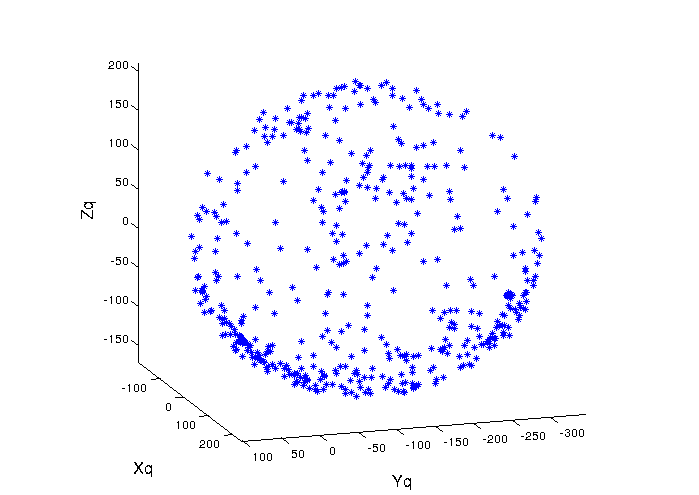
\includegraphics[width=0.5\textwidth]
		{./pics_magneto/bola.png}}
	\subfloat[Con el sensor calibrado]{\label{fig:bolacalib}
	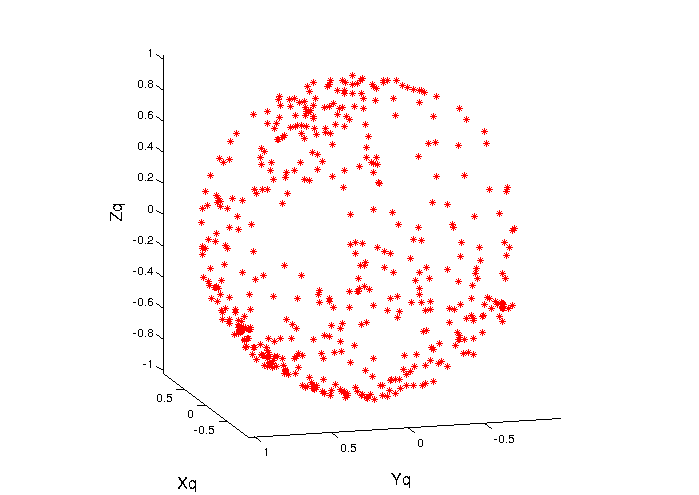
\includegraphics[width=0.5\textwidth]
		{./pics_magneto/bolacalib.png}}
  \end{center}
  \caption{Medias de campo magnético Terrestre}
\end{figure}

Para verificar que la calibraci\'on es exitosa se debe analizar con mayor detalle las caracter\'isticas de la ``esfera'' obtenida. Con los datos convertidos se procede a realizar una minimización gracias a los mínimos cuadrados para obtener las coordenadas del centro de la esfera y su radio.



Los resultados que se obtienen son:
\begin{itemize}
\item Centro de la esfera: $(-3.65\times10^{-3};-9.40\times10^{-3};1.67\times10^{-3})$
\item Radio de la esfera: $0.996$
\item Desviación estándar de la medida del radio:$\sigma = 1.54\times 10^{-2}$
\end{itemize}

A partir de dichos resultados se puede concluir que el resultado de la calibraci\'on es exitoso, ya que la representaci\'on de las medidas es pr\'acticamente una esfera de radio 1 centrada en el origen.

%\subsection{Determinaci\'on de la orientaci\'on}
%
%
%Luego de calibrado el sensor se quiere determinar la capacidad que tiene el mismo de proporcionar una adecuada orientación. Con dicho fin se utiliza la tabla larga para alinear el sensor en una dirección en particular. La ubicación donde fue realizado el experimento se encuentra marcada aproximadamente con la marca roja en la figura \ref{fig:mapa}. El objeto elegido para realizar la alineación es el que se muestra en la parte superior de la figura \ref{fig:mapa}, su ubicación es la indicada por el ``mu\~neco'' en la figura \ref{fig:mapa}.
%\begin{figure}
%  \begin{center}
%	\includegraphics[width=0.8\textwidth]
%		{./pics_magneto/mapa.png}
%	
%  \end{center}
%  \caption{Mapa de la costa de Montevideo}
%  \label{fig:mapa}
%\end{figure}
%
%Del mapa de la Intendencia de Montevideo \footnote{http://sig.montevideo.gub.uy/mapas/mapa-principal} se obtienen las coordenadas de los puntos seleccionados. El punto en que fue realizado el experimento es el (576039,6135625) y el punto con el cual se alineo es el (572118,6136415). El ángulo de la recta que une los dos puntos medido respecto del eje Sur-Norte es de $78.6^\circ$ al Oeste.\\

%TODO
%En la tabla \ref{tab:angulosconacc} se presentan los resultados de orientaci\'on obtenidos.

\end{document}

%Interesa determinar los tres \'angulos de Euler ($\theta$, $\varphi$ y $\psi$). En primer lugar se intenta utilizando exclusivamente el magnet\'ometro. En las tablas \ref{tab:angulos} se presentan los resultados obtenidos para cada m\'etodo de calibraci\'on. En la tabla se observa claramente que los resultados difieren considerablemente de lo esperado. Se confirma que el magnet\'ometro por si solo, no es suficiente para determinar la orientaci\'on del cuadric\'optero. 
%
%En reposo, los \'angulos de pitch y roll, pueden determinarse f\'acilmente gracias a la medida de aceleraci\'on. Luego de determinados dichos \'angulos se proyecta la lectura del campo magn\'etico en la base $S_1$ definida en \ref{chap:modelo_fisico}. La orientaci\'on se calcula finalmente como:
%
%$$
%\theta=atan(\vec{C_{med}}\vec{i_1}/\vec{C_{med}}\vec{j_1})
%$$
%
%Donde $C_{med}$ es el campo magn\'etico medido luego de proyectado en la base $S_1$. 
%
%Los resultados obtenidos en este caso se presentan en la tabla \ref{tab:angulosconacc}.\\
%
%
%
%
%
%
%\begin{table}
%\begin{tabular}{|p{50pt}|p{50pt}|p{50pt}|p{51pt}|p{50pt}|p{50pt}|}
%\hline
%  
%\multicolumn{2}{|p{113pt}|}{\cellcolor[gray]{0.6} $\theta$}  
%& \multicolumn{2}{|p{114pt}|}{\cellcolor[gray]{0.6} $\varphi$}
%& \multicolumn{2}{|p{113pt}|}{\cellcolor[gray]{0.6} $\psi$} 
%\\ \hline 
%   
% \multicolumn{1}{|p{50pt}|}{\cellcolor[gray]{0.7} \textbf{\'angulo te\'orico }} 
%& \multicolumn{1}{|p{50pt}|}{\cellcolor[gray]{0.8} \textbf{ángulo medido}}
%& \multicolumn{1}{|p{50pt}|}{\cellcolor[gray]{0.7} \textbf{\'angulo te\'orico }} 
%& \multicolumn{1}{|p{50pt}|}{\cellcolor[gray]{0.8} \textbf{ángulo medido}}
%& \multicolumn{1}{|p{50pt}|}{\cellcolor[gray]{0.7} \textbf{\'angulo te\'orico }} 
%& \multicolumn{1}{|p{50pt}|}{\cellcolor[gray]{0.8} \textbf{ángulo medido}}
%\\ \hline
%
% -90.20&  16.17&-90.00& 54.88&  0.00&-54.23\\ \hline
% -60.20&  27.47&-90.00& 43.92&  0.00&-26.59\\ \hline
% -45.20&  31.96&-90.00& 38.77&  0.00&-13.86\\ \hline
% -30.20&  35.82&-90.00& 33.57&  0.00& -1.70\\ \hline
%  -0.20&  43.41&-90.00& 22.75&  0.00& 22.86\\ \hline
%  89.80&  62.34&-90.00& -7.55&  0.00& 76.77\\ \hline
% -90.20& -30.76& -0.00&-19.64& 90.00& 23.46\\ \hline
% -60.20& -43.24& -0.00&-20.10& 90.00& 42.72\\ \hline
% -45.20& -45.54& -0.00&-17.55& 90.00& 53.33\\ \hline
% -30.20& -44.20& -0.00&-14.35& 90.00& 63.15\\ \hline
%  -0.20& -28.13& -0.00& -9.57& 90.00& 79.90\\ \hline
%  89.80&  46.50& -0.00&  0.62& 90.00& 61.21\\ \hline
% 179.80&  24.61& -0.00&-11.21&180.00& 84.50\\ \hline
%-150.20&  -3.43& -0.00& -9.98&180.00& 84.68\\ \hline
%-135.20& -18.96& -0.00& -9.27&180.00& 85.06\\ \hline
%-120.20& -33.05& -0.00& -8.56&180.00& 85.22\\ \hline
% -90.20& -63.76& -0.00& -6.57&180.00& 85.84\\ \hline
%  -0.20&-156.62& -0.00&-15.41&180.00& 77.69\\ \hline
%\end{tabular}
%\caption{Ángulos medidos con la primer calibración y teóricos en las distintas posiciones}
%
%
%\begin{tabular}{|p{50pt}|p{50pt}|p{50pt}|p{51pt}|p{50pt}|p{50pt}|}
%\hline
%  
%\multicolumn{2}{|p{113pt}|}{\cellcolor[gray]{0.6} $\theta$}  
%& \multicolumn{2}{|p{114pt}|}{\cellcolor[gray]{0.6} $\varphi$}
%& \multicolumn{2}{|p{113pt}|}{\cellcolor[gray]{0.6} $\psi$} 
%\\ \hline 
%   
%
% \multicolumn{1}{|p{50pt}|}{\cellcolor[gray]{0.7} \textbf{\'angulo te\'orico }} 
%& \multicolumn{1}{|p{50pt}|}{\cellcolor[gray]{0.8} \textbf{ángulo medido}}
%& \multicolumn{1}{|p{50pt}|}{\cellcolor[gray]{0.7} \textbf{\'angulo te\'orico }} 
%& \multicolumn{1}{|p{50pt}|}{\cellcolor[gray]{0.8} \textbf{ángulo medido}}
%& \multicolumn{1}{|p{50pt}|}{\cellcolor[gray]{0.7} \textbf{\'angulo te\'orico }} 
%& \multicolumn{1}{|p{50pt}|}{\cellcolor[gray]{0.8} \textbf{ángulo medido}}
%\\ \hline
%
% -90.20&  22.89&-90.00& 62.86&  0.00&-50.24\\ \hline
% -60.20&  34.83&-90.00& 50.00&  0.00&-22.52\\ \hline
% -45.20&  39.31&-90.00& 44.14&  0.00&-10.21\\ \hline
% -30.20&  43.11&-90.00& 38.26&  0.00&  1.50\\ \hline
%  -0.20&  50.58&-90.00& 25.49&  0.00& 25.90\\ \hline
%  89.80&  60.40&-90.00&-12.45&  0.00& 83.52\\ \hline
% -90.20& -24.09& -0.00&-16.70& 90.00& 19.61\\ \hline
% -60.20& -36.79& -0.00&-18.84& 90.00& 38.91\\ \hline
% -45.20& -39.90& -0.00&-17.07& 90.00& 49.95\\ \hline
% -30.20& -39.70& -0.00&-14.39& 90.00& 60.29\\ \hline
%  -0.20& -26.81& -0.00& -9.76& 90.00& 78.48\\ \hline
%  89.80&  49.40& -0.00& -1.47& 90.00& 65.71\\ \hline
% 179.80&  22.33& -0.00&-12.36&180.00& 88.71\\ \hline
%-150.20&  -4.33& -0.00&-10.00&180.00& 85.71\\ \hline
%-135.20& -18.88& -0.00& -9.31&180.00& 84.54\\ \hline
%-120.20& -31.82& -0.00& -8.90&180.00& 83.65\\ \hline
% -90.20& -59.48& -0.00& -7.79&180.00& 83.71\\ \hline
%  -0.20&-136.17& -0.00&  0.59&180.00& 84.91\\ \hline
%\end{tabular}
%\caption{Ángulos medidos con la segunda calibración y teóricos en las distintas posiciones}
%\label{tab:angulos}
%\end{table} 
%
%\begin{table}
%\begin{tabular}{|p{50pt}|p{50pt}|p{50pt}|p{51pt}|p{50pt}|p{50pt}|}
%\hline
%  
%\multicolumn{2}{|p{113pt}|}{\cellcolor[gray]{0.6} $\theta$}  
%& \multicolumn{2}{|p{114pt}|}{\cellcolor[gray]{0.6} $\varphi$}
%& \multicolumn{2}{|p{113pt}|}{\cellcolor[gray]{0.6} $\psi$} 
%\\ \hline 
%   
%
% \multicolumn{1}{|p{50pt}|}{\cellcolor[gray]{0.7} \textbf{\'angulo te\'orico }} 
%& \multicolumn{1}{|p{50pt}|}{\cellcolor[gray]{0.8} \textbf{ángulo medido}}
%& \multicolumn{1}{|p{50pt}|}{\cellcolor[gray]{0.7} \textbf{\'angulo te\'orico }} 
%& \multicolumn{1}{|p{50pt}|}{\cellcolor[gray]{0.8} \textbf{ángulo medido}}
%& \multicolumn{1}{|p{50pt}|}{\cellcolor[gray]{0.7} \textbf{\'angulo te\'orico }} 
%& \multicolumn{1}{|p{50pt}|}{\cellcolor[gray]{0.8} \textbf{ángulo medido}}
%\\ \hline
%
%-101.39&-102.65&-90.00&-90.00&  0.00&   0.00\\ \hline
% -71.39& -72.79&-90.00&-90.00&  0.00&   0.00\\ \hline
% -56.39& -58.60&-90.00&-90.00&  0.00&   0.00\\ \hline
% -41.39& -44.64&-90.00&-90.00&  0.00&   0.00\\ \hline
% -11.39& -15.33&-90.00&-90.00&  0.00&   0.00\\ \hline
%  78.61&  65.13&-90.00&-90.00&  0.00&   0.00\\ \hline
%-101.39&-100.11& -0.00& -2.21& 90.00&  92.22\\ \hline
% -71.39& -75.67& -0.00& -1.86& 90.00&  92.02\\ \hline
% -56.39& -63.05& -0.00& -1.72& 90.00&  91.97\\ \hline
% -41.39& -50.65& -0.00& -1.63& 90.00&  91.96\\ \hline
% -11.39& -23.03& -0.00& -1.55& 90.00&  92.24\\ \hline
%  78.61&  70.92& -0.00& -1.41& 90.00&  93.40\\ \hline
% 168.61& 165.02& -0.00& -0.11&180.00&-179.33\\ \hline
%-161.39&-165.54& -0.00& -0.63&180.00&-179.59\\ \hline
%-146.39&-149.33& -0.00& -0.73&180.00&-179.78\\ \hline
%-131.39&-134.53& -0.00& -0.72&180.00& 179.94\\ \hline
%-101.39&-102.08& -0.00& -0.57&180.00& 179.84\\ \hline
% -11.39& -16.00& -0.00& -0.02&180.00& 179.66\\ \hline
%\end{tabular}
%\caption{Ángulos medidos con la primer calibración y teóricos en las distintas posiciones, asistido por el aceler\'ometro}
%
%
%\begin{tabular}{|p{50pt}|p{50pt}|p{50pt}|p{51pt}|p{50pt}|p{50pt}|}
%\hline
%  
%\multicolumn{2}{|p{113pt}|}{\cellcolor[gray]{0.6} $\theta$}  
%& \multicolumn{2}{|p{114pt}|}{\cellcolor[gray]{0.6} $\varphi$}
%& \multicolumn{2}{|p{113pt}|}{\cellcolor[gray]{0.6} $\psi$} 
%\\ \hline 
%   
%
% \multicolumn{1}{|p{50pt}|}{\cellcolor[gray]{0.7} \textbf{\'angulo te\'orico }} 
%& \multicolumn{1}{|p{50pt}|}{\cellcolor[gray]{0.8} \textbf{ángulo medido}}
%& \multicolumn{1}{|p{50pt}|}{\cellcolor[gray]{0.7} \textbf{\'angulo te\'orico }} 
%& \multicolumn{1}{|p{50pt}|}{\cellcolor[gray]{0.8} \textbf{ángulo medido}}
%& \multicolumn{1}{|p{50pt}|}{\cellcolor[gray]{0.7} \textbf{\'angulo te\'orico }} 
%& \multicolumn{1}{|p{50pt}|}{\cellcolor[gray]{0.8} \textbf{ángulo medido}}
%\\ \hline
%
%-101.39&-110.21&-90.00&-90.00&  0.00&   0.00\\ \hline
% -71.39& -77.27&-90.00&-90.00&  0.00&   0.00\\ \hline
% -56.39& -62.03&-90.00&-90.00&  0.00&   0.00\\ \hline
% -41.39& -47.03&-90.00&-90.00&  0.00&   0.00\\ \hline
% -11.39& -14.40&-90.00&-90.00&  0.00&   0.00\\ \hline
%  78.61&  73.61&-90.00&-90.00&  0.00&   0.00\\ \hline
%-101.39&-108.27& -0.00& -2.21& 90.00&  92.22\\ \hline
% -71.39& -80.63& -0.00& -1.86& 90.00&  92.02\\ \hline
% -56.39& -66.41& -0.00& -1.72& 90.00&  91.97\\ \hline
% -41.39& -52.67& -0.00& -1.63& 90.00&  91.96\\ \hline
% -11.39& -23.42& -0.00& -1.55& 90.00&  92.24\\ \hline
%  78.61&  66.18& -0.00& -1.41& 90.00&  93.40\\ \hline
% 168.61& 165.14& -0.00& -0.11&180.00&-179.33\\ \hline
%-161.39&-164.83& -0.00& -0.63&180.00&-179.59\\ \hline
%-146.39&-149.40& -0.00& -0.73&180.00&-179.78\\ \hline
%-131.39&-135.93& -0.00& -0.72&180.00& 179.94\\ \hline
%-101.39&-107.43& -0.00& -0.57&180.00& 179.84\\ \hline
% -11.39& -22.85& -0.00& -0.02&180.00& 179.66\\ \hline
%\end{tabular}
%\caption{Ángulos medidos con la segunda calibración y teóricos en las distintas posiciones, asistido por el aceler\'ometro}
%\label{tab:angulosacc}
%\end{table} 
%
%En este caso los \'angulos encontrados se asemejan en mayor medida a los resultados te\'oricos.  
%
%
%
%El error promedio obtenido con el primer m\'etodo de calibraci\'on es $\mu_1=-61^\circ$, la desviación estándar obtenida es $\sigma_1=3.83^\circ$, mientras que para el segundo método de calibración tenemos que $\mu_2=-7.10^\circ$, la desviación estándar obtenida es $\sigma_2=3.28^\circ$.\\
%
%Cabe aclarar que la exactitud de los resultados obtenidos para las seis primeras medidas en los \'angulos de pitch y roll, se debe a un ajuste realizado para cubrirse frente a la situaci\'on de \emph{gimbal lock}. El an\'alisis del error cometido en la medida de los \'angulos de pitch y roll puede encontrarse en el cap\'itulo \ref{chap:acelerometro}.\\
%
%
%
%En ambos casos se obtiene un error promedio distinto de cero. Con cualquier método de ajuste que se elija se deberá restar a la medida realizada el error promedio. Lo más adecuado parece ser elegir el método que tiene una desviación estándar menor. Por dicho motivo volvemos a escoger el segundo método. 
%
%
%
%
%
%
%
